\documentclass[a4paper]{article}

%%%%%%%%%%%%%%%%%%%%%%%%%%%%%%%%%%%%%%%%%%%%%%%%%%%%%%%%%%%%%%%
%%%
%%% Zuerst laden wir ein paar nützliche Pakete
%%%
%%%%%%%%%%%%%%%%%%%%%%%%%%%%%%%%%%%%%%%%%%%%%%%%%%%%%%%%%%%%%%%

%%%%%%%%%%%%%%%%%%%%%%%%%%%%%%%%%%%%%%%%%%%%%%%%%%%%%%%%%%%%%%%
% AMS-Pakete: mathematische Fonts
%%%%%%%%%%%%%%%%%%%%%%%%%%%%%%%%%%%%%%%%%%%%%%%%%%%%%%%%%%%%%%%
\usepackage{amsmath}
\usepackage{amssymb}
%%%%%%%%%%%%%%%%%%%%%%%%%%%%%%%%%%%%%%%%%%%%%%%%%%%%%%%%%%%%%%%
% Babel-Paket: Silbentrennung (Deutsch/neue Rechtschtreibung)
%%%%%%%%%%%%%%%%%%%%%%%%%%%%%%%%%%%%%%%%%%%%%%%%%%%%%%%%%%%%%%%
\usepackage[english,ngerman]{babel}
%%%%%%%%%%%%%%%%%%%%%%%%%%%%%%%%%%%%%%%%%%%%%%%%%%%%%%%%%%%%%%%
% fontenc & inputenc: Umlaute in UTF8 eingeben
%%%%%%%%%%%%%%%%%%%%%%%%%%%%%%%%%%%%%%%%%%%%%%%%%%%%%%%%%%%%%%%
\usepackage[T1]{fontenc}
\usepackage[utf8]{inputenc}
%%%%%%%%%%%%%%%%%%%%%%%%%%%%%%%%%%%%%%%%%%%%%%%%%%%%%%%%%%%%%%%
% graphicx: Graphiken einbinden
%%%%%%%%%%%%%%%%%%%%%%%%%%%%%%%%%%%%%%%%%%%%%%%%%%%%%%%%%%%%%%%
\usepackage{graphicx}
%%%%%%%%%%%%%%%%%%%%%%%%%%%%%%%%%%%%%%%%%%%%%%%%%%%%%%%%%%%%%%%
% color: farbige Texte, Hintergründe, Links, etcpp.
%%%%%%%%%%%%%%%%%%%%%%%%%%%%%%%%%%%%%%%%%%%%%%%%%%%%%%%%%%%%%%%
\usepackage{color}
%%%%%%%%%%%%%%%%%%%%%%%%%%%%%%%%%%%%%%%%%%%%%%%%%%%%%%%%%%%%%%%
% tikz/pgfplots: Bilder in LaTeX zeichnen
%%%%%%%%%%%%%%%%%%%%%%%%%%%%%%%%%%%%%%%%%%%%%%%%%%%%%%%%%%%%%%%
\usepackage{tikz}
\usetikzlibrary{decorations.pathmorphing,patterns,calc}
\usepackage{pgfplots}
\pgfplotsset{compat=1.12}
\usepackage{calculus}
%%%%%%%%%%%%%%%%%%%%%%%%%%%%%%%%%%%%%%%%%%%%%%%%%%%%%%%%%%%%%%%
% geometry: bessere Ausnutzung des verfügbaren Platzes
%%%%%%%%%%%%%%%%%%%%%%%%%%%%%%%%%%%%%%%%%%%%%%%%%%%%%%%%%%%%%%%
\usepackage[a4paper,includeheadfoot,margin=2.54cm]{geometry}
%%%%%%%%%%%%%%%%%%%%%%%%%%%%%%%%%%%%%%%%%%%%%%%%%%%%%%%%%%%%%%%
% epstopdf: automatische Umwandlung von EPS nach PDF
%%%%%%%%%%%%%%%%%%%%%%%%%%%%%%%%%%%%%%%%%%%%%%%%%%%%%%%%%%%%%%%
\usepackage{epstopdf}

%%%%%%%%%%%%%%%%%%%%%%%%%%%%%%%%%%%%%%%%%%%%%%%%%%%%%%%%%%%%%%%
%%%
%%% Nun definieren wir ein paar hilfreiche Dinge
%%%
%%%%%%%%%%%%%%%%%%%%%%%%%%%%%%%%%%%%%%%%%%%%%%%%%%%%%%%%%%%%%%%
%
% Generelles Umstellen des Doppelpunktes auf dieselbe
% Linie wie das Gleichheitszeichen. Aus de-tex-faq, Teil 8,
% Makro von Donald Arseneau
%
\mathchardef\ordinarycolon\mathcode`\:
\mathcode`\:=\string"8000
\begingroup \catcode`\:=\active
  \gdef:{\mathrel{\mathop\ordinarycolon}}
\endgroup
%%
%% definition of Perlis mathclap etcpp.
%%
% For comparison, the existing overlap macros:
% \def\llap#1{\hbox to 0pt{\hss#1}}
% \def\rlap#1{\hbox to 0pt{#1\hss}}
\def\clap#1{\hbox to 0pt{\hss#1\hss}}
\def\mathllap{\mathpalette\mathllapinternal}
\def\mathrlap{\mathpalette\mathrlapinternal}
\def\mathclap{\mathpalette\mathclapinternal}
\def\mathllapinternal#1#2{%
  \llap{$\mathsurround=0pt#1{#2}$}}
\def\mathrlapinternal#1#2{%
  \rlap{$\mathsurround=0pt#1{#2}$}}
\def\mathclapinternal#1#2{%
  \clap{$\mathsurround=0pt#1{#2}$}}
%%
%% end of perlis stuff
%%
%%
%% definition of inverse diagonal dots (iddots)
%%
\makeatletter
\def\iddots{\mathinner{\mkern1mu\raise\p@%
    \hbox{.}\mkern2mu\raise4\p@\hbox{.}\mkern2mu%
    \raise7\p@\vbox{\kern7\p@\hbox{.}}\mkern1mu}}
\makeatother
%%%\def\ddots{\mathinner{\mkern1mu\raise7\p@\vbox%
%%%{\kern7\p@\hbox{.}} \mkern2mu\raise4\p@\hbox{.}%
%%%\mkern2mu\raise\p@\hbox{.}\mkern1mu}}
%
% TIME OF DAY (Nelson H. F. Beebe :-)
%
\newcount\hh
\newcount\mm
\mm=\time
\hh=\time
\divide\hh by 60
\divide\mm by 60
\multiply\mm by 60
\mm=-\mm
\advance\mm by \time
\def\hhmm{\number\hh:\ifnum\mm<10{}0\fi\number\mm}
%
% Use it like this in a LaTeX document:
%
%        \date{\today{ }\hhmm}
%
%%%%%%%%%%%%%%%%%%%%%%%%%%%%%%%%%%%%%%%%%%%%%%%%%%%%%%%%%%%%%%%
%%%
%%% Wir definieren Makros für fette Buchstaben
%%%
%%%%%%%%%%%%%%%%%%%%%%%%%%%%%%%%%%%%%%%%%%%%%%%%%%%%%%%%%%%%%%%
%%% small bold letters
\newcommand{\bfa}{{\mathbf a}}
\newcommand{\bfb}{{\mathbf b}}
\newcommand{\bfc}{{\mathbf c}}
\newcommand{\bfd}{{\mathbf d}}
\newcommand{\bfe}{{\mathbf e}}
\newcommand{\bff}{{\mathbf f}}
\newcommand{\bfg}{{\mathbf g}}
\newcommand{\bfh}{{\mathbf h}}
\newcommand{\bfi}{{\mathbf i}}
\newcommand{\bfj}{{\mathbf j}}
\newcommand{\bfk}{{\mathbf k}}
\newcommand{\bfl}{{\mathbf l}}
\newcommand{\bfm}{{\mathbf m}}
\newcommand{\bfn}{{\mathbf n}}
\newcommand{\bfo}{{\mathbf o}}
\newcommand{\bfp}{{\mathbf p}}
\newcommand{\bfq}{{\mathbf q}}
\newcommand{\bfr}{{\mathbf r}}
\newcommand{\bfs}{{\mathbf s}}
\newcommand{\bft}{{\mathbf t}}
\newcommand{\bfu}{{\mathbf u}}
\newcommand{\bfv}{{\mathbf v}}
\newcommand{\bfw}{{\mathbf w}}
\newcommand{\bfx}{{\mathbf x}}
\newcommand{\bfy}{{\mathbf y}}
\newcommand{\bfz}{{\mathbf z}}
%%% capital bold letters
\newcommand{\bfA}{{\mathbf A}}
\newcommand{\bfAT}{{\mathbf A}\kern-.15em^{\mathsf{T}}}
\newcommand{\bfB}{{\mathbf B}}
\newcommand{\bfC}{{\mathbf C}}
\newcommand{\bfD}{{\mathbf D}}
\newcommand{\bfE}{{\mathbf E}}
\newcommand{\bfF}{{\mathbf F}}
\newcommand{\bfG}{{\mathbf G}}
\newcommand{\bfH}{{\mathbf H}}
\newcommand{\bfI}{{\mathbf I}}
\newcommand{\bfJ}{{\mathbf J}}
\newcommand{\bfK}{{\mathbf K}}
\newcommand{\bfL}{{\mathbf L}}
\newcommand{\bfM}{{\mathbf M}}
\newcommand{\bfN}{{\mathbf N}}
\newcommand{\bfO}{{\mathbf O}}
\newcommand{\bfP}{{\mathbf P}}
\newcommand{\bfQ}{{\mathbf Q}}
\newcommand{\bfR}{{\mathbf R}}
\newcommand{\bfS}{{\mathbf S}}
\newcommand{\bfT}{{\mathbf T}}
\newcommand{\bfU}{{\mathbf U}}
\newcommand{\bfV}{{\mathbf V}}
\newcommand{\bfW}{{\mathbf W}}
\newcommand{\bfX}{{\mathbf X}}
\newcommand{\bfY}{{\mathbf Y}}
\newcommand{\bfZ}{{\mathbf Z}}
%% extra bold symbols
\newcommand{\bfell}{{\boldsymbol{\ell}}}
\newcommand{\bfLambda}{{\boldsymbol{\Lambda}}}
\newcommand{\bfSigma}{{\boldsymbol{\Sigma}}}
\newcommand{\bfnu}{{\boldsymbol{\nu}}}
\newcommand{\bfphi}{{\boldsymbol{\phi}}}
\newcommand{\bfalpha}{{\boldsymbol{\alpha}}}
\newcommand{\bfbeta}{{\boldsymbol{\beta}}}
\newcommand{\bfhatbeta}{{\boldsymbol{\widehat{\beta}}}}
\newcommand{\bfomega}{{\boldsymbol{\omega}}}
\newcommand{\bfrho}{{\boldsymbol{\rho}}}
\newcommand{\bfmu}{{\boldsymbol{\mu}}}
\newcommand{\bfchecknu}{{\boldsymbol{\check{\nu}}}}
\newcommand{\bfhatnu}{{\boldsymbol{\widehat{\nu}}}}
%%%%%%%%%%%%%%%%%%%%%%%%%%%%%%%%%%%%%%%%%%%%%%%%%%%%%%%%%%%%%%%
%%%
%%% Zum Setzen von Sätzen, Beweisen, Lemmata, Definitionen
%%%
%%%%%%%%%%%%%%%%%%%%%%%%%%%%%%%%%%%%%%%%%%%%%%%%%%%%%%%%%%%%%%%
\usepackage{amsthm}
\newtheorem{theorem}{Satz}[section]
\newtheorem{lemma}[theorem]{Lemma}%[section]
\newtheorem{corollary}[theorem]{Korollar}%[section]
\theoremstyle{definition}
\newtheorem{definition}[theorem]{Definition}%[section]
\newtheorem{remark}[theorem]{Bemerkung}%[section]
%%%%%%%%%%%%%%%%%%%%%%%%%%%%%%%%%%%%%%%%%%%%%%%%%%%%%%%%%%%%%%%
%%%
%%% Mathematische Operatoren in \textsf
%%%
%%%%%%%%%%%%%%%%%%%%%%%%%%%%%%%%%%%%%%%%%%%%%%%%%%%%%%%%%%%%%%%
\renewcommand{\det}{\mathop{\mathsf{det}}}
\newcommand{\adj}{\mathop{\mathsf{adj}}}
\renewcommand{\dim}{\mathop{\mathsf{dim}}}
\renewcommand{\deg}{\mathop{\mathsf{deg}}}
\renewcommand{\max}{\mathop{\mathsf{max}}}
\renewcommand{\min}{\mathop{\mathsf{min}}}
\newcommand{\argmin}{\mathop{\mathsf{arg\ min}}}
\newcommand{\diag}{\mathop{\mathsf{diag}}}
\newcommand{\triu}{\mathop{\mathsf{triu}}}
\newcommand{\tril}{\mathop{\mathsf{tril}}}
\newcommand{\ones}{\mathop{\mathsf{ones}}}
\newcommand{\zeros}{\mathop{\mathsf{zeros}}}
\newcommand{\eye}{\mathop{\mathsf{eye}}}
\newcommand{\conj}{\mathop{\mathsf{conj}}}
\newcommand{\norm}{\mathop{\mathsf{norm}}}
\newcommand{\Mod}{\mathop{\mathsf{mod}}}
\newcommand{\spdiags}{\mathop{\mathsf{spdiags}}}
\newcommand{\circshift}{\mathop{\mathsf{circshift}}}
\newcommand{\fliplr}{\mathop{\mathsf{fliplr}}}
\newcommand{\logical}{\mathop{\mathsf{logical}}}
\newcommand{\Summe}{\mathop{\mathsf{sum}}}
\newcommand{\sign}{\mathop{\mathsf{sign}}}
\newcommand{\cumprod}{\mathop{\mathsf{cumprod}}}
\renewcommand{\limsup}{\mathop{\mathsf{lim\ sup}}}
\newcommand{\spur}{\mathop{\mathsf{spur}}}
\renewcommand{\vec}{\mathop{\mathsf{vec}}}
\newcommand{\spec}{\mathop{\mathsf{spec}}}
\newcommand{\speceps}{\mathop{\mathsf{spec}_{\epsilon}}}
\newcommand{\Bild}{\mathop{\mathsf{Bild}}}
\newcommand{\Kern}{\mathop{\mathsf{Kern}}}
\newcommand{\Span}{\mathop{\mathsf{span}}}
\newcommand{\Index}{\mathop{\mathsf{Index}}}
\newcommand{\Rang}{\mathop{\mathsf{Rang}}}
% hack for seto = searrow in small
\newcommand{\seto}{\mathop{\scalebox{.5}{$\searrow$}}}
\newcommand{\neto}{\mathop{\scalebox{.5}{$\nearrow$}}}
% end of hack for seto = searrow in small
%%%%%%%%%%%%%%%%%%%%%%%%%%%%%%%%%%%%%%%%%%%%%%%%%%%%%%%%%%%%%%%
%%%
%%% kleiner Hack, um Einträge in Matrizen anders auszurichten
%%%
%%%%%%%%%%%%%%%%%%%%%%%%%%%%%%%%%%%%%%%%%%%%%%%%%%%%%%%%%%%%%%%
\makeatletter
\renewcommand*\env@matrix[1][*\c@MaxMatrixCols c]{%
  \hskip -\arraycolsep
  \let\@ifnextchar\new@ifnextchar
  \array{#1}}
\makeatother
%%%%%%%%%%%%%%%%%%%%%%%%%%%%%%%%%%%%%%%%%%%%%%%%%%%%%%%%%%%%%%%
%%%
%%% Wir wollen Matlab-Beispielprogramme einbinden
%%%
%%%%%%%%%%%%%%%%%%%%%%%%%%%%%%%%%%%%%%%%%%%%%%%%%%%%%%%%%%%%%%%
\usepackage{listings}
\definecolor{hellgrau}{rgb}{0.90,0.90,0.90}
\definecolor{commentcol}{rgb}{0.0823,.4902,0.0}
\lstset{language=Matlab,
        basicstyle={\footnotesize\ttfamily},
        keywordstyle={\sffamily\bfseries},
        tabsize=2,
        escapechar=\#,
        numbers=left,
        numberstyle=\tt,
        stepnumber=1,
        numbersep=7pt,
        breaklines=true,
        frame=single,
        frameround=ffff,
        commentstyle=\color{commentcol},
        backgroundcolor=\color{hellgrau}
}
%%%%%%%%%%%%%%%%%%%%%%%%%%%%%%%%%%%%%%%%%%%%%%%%%%%%%%%%%%%%%%%
%%%
%%% Wir wollen verlinkte PDF-Dateien, dazu ein paar Zeilen
%%%
%%%%%%%%%%%%%%%%%%%%%%%%%%%%%%%%%%%%%%%%%%%%%%%%%%%%%%%%%%%%%%%
\usepackage{ifpdf}
\ifpdf
\usepackage[pdftex]{hyperref}
\usepackage{thumbpdf}
\else
\usepackage[dvips,ps2pdf,naturalnames]{hyperref}
\fi
\definecolor{mycolor}{rgb}{.08,.12,.71}
\hypersetup{%
  pdftitle     = {Proseminar über numerische lineare Algebra},
  pdfsubject   = {Proseminar Mathematik},
  pdfkeywords  = {Proseminar, Mathematik, numerische lineare Algebra,
    TUHH},
  pdfauthor    = {\textcopyright\ Jens-Peter M. Zemke 2017},
  baseurl      = {http://www.mat.tuhh.de/home/jpmzemke/},
  pdfstartview = {FitH},
  pdfview      = {FitH},
  linkcolor    = mycolor,     % links to same page
  urlcolor     = mycolor,     % links to URLs
  citecolor    = mycolor,     % links to citations
  breaklinks   = true,       % links may (line) break
  colorlinks   = true,
  citebordercolor=0 0 0,  % color for \cite
  filebordercolor=0 0 0,
  linkbordercolor=0 0 0,
  menubordercolor=0 0 0,
  urlbordercolor=0 0 0,
  pdfhighlight=/P,   % moeglich /I, /P, ...
  pdfborder=0 0 0,   % keine Box um die Links!
}
%%%%%%%%%%%%%%%%%%%%%%%%%%%%%%%%%%%%%%%%%%%%%%%%%%%%%%%%%%%%%%%
%%%
%%% Zum Setzen von Algorithmen
%%%
%%%%%%%%%%%%%%%%%%%%%%%%%%%%%%%%%%%%%%%%%%%%%%%%%%%%%%%%%%%%%%%
\usepackage{algorithmic}
\renewcommand{\algorithmiccomment}[2]{\hfill\rlap{\texttt{\%
      #1}}\phantom{\texttt{\% #2}}}
\renewcommand{\algorithmicrequire}{\textsc{Eingabe:}}
\renewcommand{\algorithmicensure}{\textsc{Ausgabe:}}
\usepackage[Algorithmus]{algorithm}
\numberwithin{algorithm}{section}
%%%
\usepackage{hypcap}
\renewcommand{\hypcapspace}{0pt}
%%%%%%%%%%%%%%%%%%%%%%%%%%%%%%%%%%%%%%%%%%%%%%%%%%%%%%%%%%%%%%%
%%%
%%% … endlich geht es los!
%%%
%%%%%%%%%%%%%%%%%%%%%%%%%%%%%%%%%%%%%%%%%%%%%%%%%%%%%%%%%%%%%%%
\begin{document}

\title{\Huge \textbf{Proseminar über numerische lineare Algebra}}
\author{\textsc{Rustam Magomedov}}
\date{\today}
\maketitle%

\tableofcontents%

\newpage

\phantomsection
\addcontentsline{toc}{section}{Tabellenverzeichnis}%
\listoftables%
\phantomsection
\addcontentsline{toc}{section}{Abbildungsverzeichnis}%
\listoffigures%
\phantomsection
\addcontentsline{toc}{section}{Algorithmenverzeichnis}%
\listof{algorithm}{Algorithmenverzeichnis}%

\newpage

\section{Grundlegendes}
\label{sec:Grundlegendes}

Im „Proseminar über numerische lineare Algebra“ behandeln wir einfache
Themen aus der numerischen linearen Algebra. Wir richten uns nach dem
Buch~\cite{Watkins:2002}, welches über unsere Bibliothek als E-Book
verfügbar ist. Es werden bis zu 36 Abschnitte aus diesem Buch auf die
bis zu 36 Teilnehmer verteilt. Jeder Teilnehmer erarbeitet auf der
Grundlage dieses \LaTeX-Dokumentes eine kleine Ausarbeitung (zwischen
$3$ und $15$ Seiten) zu „seinem“ Thema, programmiert nötige oder
selbst erdachte Algorithmen in \textsc{Matlab}, und führt in einem
halbstündigen mittels der \LaTeX-Beamer-Klasse erarbeiteten Vortrag
„sein“ Thema vor. Pro Termin werden wir drei Vorträge haben, die
wöchentlichen Treffen finden ab dem 10.04.2017 montags von 17:00 Uhr
bis 18:30 Uhr im Channel Harburg in Raum CH4-0.08 statt. Unser erstes
Treffen findet allerdings bereits am 03.04.2017 in Raum H0.07 statt.

\subsection{Das mathematische Thema}
\label{sec:Grundlegendes_Thema}

Das Thema sind die ersten Kapitel des Buches~\cite{Watkins:2002}. In
diesem Buch geht es um die numerische lineare Algebra, das ist die
lineare Algebra, wie man sie auf einem Rechner ausführt. Dabei werden
uns die Themen aus der linearen Algebra I und II wieder begegnen,
beginnend mit
\begin{itemize}
\item dem Gauß'schen Eliminationsverfahren,
\item der Sensitivität der Lösung/des Lösungsprozesses linearer
  Gleichungssysteme bei (unvermeidbaren) Rundungsfehlern,
\item Ausgleichsproblemen und orthogonalen Matrizen nebst dem
  Gram-Schmidt'schen Orthonormalisierungsverfahren,
\item der Singulärwertzerlegung (kurz: SVD) und ihrer Berechnung,
\item der Berechnung von Eigenwerten und Eigenvektoren,
\item (möglicherweise) noch unbekannten iterativen Methoden zur
  Lösung linearer Gleichungssysteme.
\end{itemize}
Sie lernen also alle noch etwas Nützliches!

\subsection{Die Ausarbeitung in \LaTeX}
\label{sec:Grundlegendes_Ausarbeitung_in_LaTeX}

Sie schreiben eine kurze Ausarbeitung zu Ihrem Thema unter Verwendung
des diesem Dokument zugrunde liegenden \LaTeX-Quellcodes. \LaTeX\ ist
eine Sammlung von Makros von Leslie Lamport zu Donald Knuths
\TeX-Paket, welche gerade für mathematische Themen enorme Vorteile
bietet. Solcherart sind Sie danach gut gewappnet, um Ihre Bachelor-
und Masterarbeiten an der TUHH zu schreiben. Es gibt viele gute Bücher
zu \LaTeX, und natürlich gibt es da noch das große weite Internet.

In \LaTeX\ können Sie schnell mathematische Formeln wie
$f(x):=x^2-\sin(x)$ oder Terme wie $\int_0^1f(x)\,dx$ setzen, Sie
können auch rasch abgesetzte und automatisch nummerierte Formeln
setzen, wie das Beispiel
\begin{equation}
  \label{eq:eine_erste_abgesetzte_Formel}
  \begin{pmatrix}
    1 & 2 & 3\\
    4 & 5 & 6\\
    7 & 8 & 9\\
  \end{pmatrix}
  \begin{pmatrix}[r]
    1 \\ -2 \\ 1\\
  \end{pmatrix} = 
  \begin{pmatrix}
    0 \\ 0 \\ 0\\
  \end{pmatrix} \quad\Leftrightarrow\quad
  \bfA\bfx=\bfo
\end{equation}
zeigt. Ab jetzt können Sie auf diese Formel automatisch zugreifen,
indem Sie den Befehl \verb|\eqref| verwenden, die
Formel~\eqref{eq:eine_erste_abgesetzte_Formel} wird dann korrekt
referenziert und verlinkt, egal wie viele Formeln Sie vorher oder
nachher noch einfügen. Wenn Sie die Verlinkung etwas schöner gestalten
wollen, können Sie mit dem \verb|\hyperref|-Befehl das Resultat
    „\hyperref[eq:eine_erste_abgesetzte_Formel]%
    {Formel~(\ref*{eq:eine_erste_abgesetzte_Formel})}“ erzielen.

Wollen Sie mehrere Formeln gruppieren, bietet sich z.~B. die Umgebung
\texttt{align} an,
\begin{align}
  \label{eq:erste_Zeile_gruppierter_Formeln}
  a(x) &= x^2+4, & b(x) &= x^3-4x^2, \\
  \label{eq:zweite_Zeile_gruppierter_Formeln}
  c(x) &= x^2+x, & d(x) &= x^3+13, \\
  \label{eq:dritte_Zeile_gruppierter_Formeln}
  e(x) &= x^2+4x, & f(x) &= x^5-12x^3.
\end{align}
Hier haben jetzt alle Zeilen eine Formelnummer bekommen, einzelne
Formelnummern können Sie mittels \verb|\notag| unterdrücken. Jetzt
können Sie auf die einzelnen Zeilen zugreifen,
\begin{enumerate}
\item die erste Zeile hat die
  Nummer~\eqref{eq:erste_Zeile_gruppierter_Formeln},
\item die zweite Zeile hat die
  Nummer~\eqref{eq:zweite_Zeile_gruppierter_Formeln},
\item die dritte Zeile hat die
  Nummer~\eqref{eq:dritte_Zeile_gruppierter_Formeln}.
\end{enumerate}
Wollen Sie die Nummern zusammenfassen, so bietet sich zusätzlich die
Umgebung \texttt{subequations} an:
\begin{subequations}
  \label{eq:gruppierte_Formeln}
  \begin{align}
    \label{eq:erste_Zeile_gruppierter_Formeln_a}
    a(x) &= x^2+4, & b(x) &= x^3-4x^2, \\
    \label{eq:zweite_Zeile_gruppierter_Formeln_b}
    c(x) &= x^2+x, & d(x) &= x^3+13, \\
    \label{eq:dritte_Zeile_gruppierter_Formeln_c}
    e(x) &= x^2+4x, & f(x) &= x^5-12x^3.
  \end{align}
\end{subequations}
Nun können Sie auf eine einzelne Zeile, zum Beispiel die zweite,
also~\eqref{eq:zweite_Zeile_gruppierter_Formeln_b} zugreifen, oder auf
den gesamten Formelblock~\eqref{eq:gruppierte_Formeln}.

Tabellen lassen sich auch in \LaTeX\ erzeugen, so beschreibt die
\hyperref[Tab:Themen]{Tabelle~\ref*{Tab:Themen}} auf
Seite~\pageref{Tab:Themen} die Aufteilung der Themen~\cite[Kapitel
1--5]{Watkins:2002} auf die einzelnen Teilnehmer, sowie durch
farbliche Hervorhebung die Einteilung in je drei Themen zu einem
Block, welcher aus drei halbstündigen Vorträgen besteht und an einem
Termin stattfinden wird.

\begin{table}[htb]
\begin{tabular}{|r|l|l|}\hline
\textbf{No.} & \textbf{Vor- und Nachname} & \textbf{Thema} \\\hline
\multicolumn{3}{|l|}{Kapitel 1: Gaussian Elimination and Its Variants.}\\\hline
  \textcolor{blue}{1}&&
1.1 Matrix Multiplication.\\\hline
  \textcolor{blue}{2}&&
1.2 Systems of Linear Equations.\\\hline
  \textcolor{blue}{3}&&
1.3 Triangular Systems.\\\hline
  \textcolor{red}{4}&&
1.4 Positive Definite Systems; Cholesky Decomposition.\\\hline
  \textcolor{red}{5}&&
1.5 Banded Positive Definite Systems.\\\hline
  \textcolor{red}{6}&&
1.6 Sparse Positive Definite Systems.\\\hline
  \textcolor{black}{7}&&
1.7 Gaussian Elimination and the LU Decomposition.\\\hline
  \textcolor{black}{8}&&
1.8 Gaussian Elimination with Pivoting.\\\hline
  \textcolor{black}{9}&&
1.9 Sparse Gaussian Elimination.\\\hline
\multicolumn{3}{|l|}{Kapitel 2: Sensitivity of Linear Systems.}\\\hline
  \textcolor{blue}{10}&&
2.1 Vector and Matrix Norms.\\\hline
  \textcolor{blue}{11}&&
2.2 Condition Numbers.\\\hline
  \textcolor{blue}{12}&&
2.3 Perturbing the Coefficient Matrix.\\\hline
  \textcolor{red}{13}&&
2.4 A Posteriori Error Analysis Using the Residual.\\\hline
  \textcolor{red}{14}&&
2.5 Roundoff Errors; Backward Stability.\\\hline
  \textcolor{red}{15}&&
2.6 Propagation of Roundoff Errors.\\\hline
  \textcolor{black}{16}&&
2.7 Backward Error Analysis of Gaussian Elimination.\\\hline
  \textcolor{black}{17}&&
2.8 Scaling.\\\hline
  \textcolor{black}{18}&&
2.9 Componentwise Sensitivity Analysis.\\\hline
\multicolumn{3}{|l|}{Kapitel 3: The Least Squares Problem.}\\\hline
  \textcolor{blue}{19}&&
3.1 The Discrete Least Squares Problem.\\\hline
  \textcolor{blue}{20}&&
3.2 Orthogonal Matrices, Rotators and Reflectors.\\\hline
  \textcolor{blue}{21}&&
3.3 Solution of the Least Squares Problem.\\\hline
  \textcolor{red}{22}&&
3.4 The Gram-Schmidt Process.\\\hline
  \textcolor{red}{23}&&
3.5 Geometric Approach.\\\hline
  \textcolor{red}{24}&&
3.6 Updating the QR Decomposition.\\\hline
\multicolumn{3}{|l|}{Kapitel 4: The Singular Value Decomposition.}\\\hline
  \textcolor{black}{25}&&
4.1 Introduction.\\\hline
  \textcolor{black}{26}&&
4.2 Some Basic Applications of Singular Values.\\\hline
  \textcolor{black}{27}&&
4.3 The SVD and the Least Squares Problem.\\\hline
  \textcolor{blue}{28}&&
4.4 Sensitivity of the Least Squares Problem.\\\hline
\multicolumn{3}{|l|}{Kapitel 5: Eigenvalues and Eigenvectors I.}\\\hline
  \textcolor{blue}{29}&&
5.1 Systems of Differential Equations.\\\hline
  \textcolor{blue}{30}&&
5.2 Basic Facts.\\\hline
  \textcolor{red}{31}&&
5.3 The Power Method and Some Simple Extensions.\\\hline
  \textcolor{red}{32}&&
5.4 Similarity Transforms.\\\hline
  \textcolor{red}{33}&&
5.5 Reduction to Hessenberg and Tridiagonal Forms.\\\hline
  \textcolor{black}{34}&&
5.6 The QR Algorithm.\\\hline
  \textcolor{black}{35}&&
5.7 Use of the QR Algorithm to Calculate Eigenvectors.\\\hline
  \textcolor{black}{36}&&
5.8 The SVD Revisted.\\\hline
\end{tabular}
  \caption{\label{Tab:Themen} Tabelle der Themen, farblich sortiert
    nach Terminen}
\end{table}

Sie können in \LaTeX\ auch Bilder erzeugen oder einbinden. Als
Beispiel eines eingebundenen Bildes finden Sie im
       \hyperref[sec:Grundlegendes_Matlab]%
{Abschnitt~\ref*{sec:Grundlegendes_Matlab}} über \textsc{Matlab} die
\hyperref[Abb:Eigenwerte]{Abbildung~\ref*{Abb:Eigenwerte}} auf
Seite~\pageref{Abb:Eigenwerte}. Um ein Bild zu zeichnen, können Sie
dank PGF/TikZ direkt in \LaTeX\ zeichnen, siehe
\hyperref[Abb:Schach]{Abbildung~\ref*{Abb:Schach}}. Sie können auch
direkt innerhalb des Textes ein kleines Bild, zum Beispiel
\tikz[baseline=1pt,scale=.7]{%
  \draw[->] (-.1,0)--(.4,0);
  \draw[->] (0,-.1)--(0,.4);
  \fill[green]
    (0,0)--(.3,.3)--(.3,0)--cycle;
  \draw[thick] (0,0)--(.3,.3)--(.3,0)--cycle;
  \draw (-.1,-.1)--(.4,.4);
}, einfügen.

\begin{figure}[htb]
\begin{center}
\tikz[baseline=1.9cm,scale=0.5]{
  \foreach \x in {0,...,7} \foreach \y in {0,...,7}
  {
    \pgfmathparse{int(mod(\x+\y,2))}
    \ifnum\pgfmathresult=0{\draw[fill] (\x,\y)
      rectangle (\x+1,\y+1);}
    \else{\draw (\x,\y)
      rectangle (\x+1,\y+1);}
    \fi
  }
}
\end{center}
\caption{\label{Abb:Schach} Ein Schachbrett mittels PGF/TikZ.}
\end{figure}

Sie können in \LaTeX\ auch Algorithmen setzen, als Beispiel sei auf
die Implementation des Gram-Schmidt'schen
Orthonormalisierungsverfahrens angewandt auf die Spalten der Matrix
$\bfA\in\mathbb{R}^{m\times n}$ mit $\Rang(\bfA)=n$ zur Erzeugung
einer Orthonormalbasis, gespeichert in den Spalten der Matrix
$\bfQ\in\mathbb{R}^{m\times n}$ in
\hyperref[alg:CGS]{Algorithmus~\ref*{alg:CGS}} verwiesen, welche
gleichzeitig eine QR-Zerlegung berechnet, wobei die obere
Dreiecksmatrix $\bfR\in\mathbb{R}^{n\times n}$ die
Orthonormalisierungsgrößen enthält.

\begin{algorithm}
  \caption{Das klassische Gram-Schmidt-Verfahren%
    \label{alg:CGS}}
  \begin{algorithmic}[1]
    \REQUIRE $\bfA\in\mathbb{R}^{m\times n}$ mit $\Rang(\bfA)=n$.
    \ENSURE $\bfQ\in\mathbb{R}^{m\times n}$ orthonormal und
    $\bfR\in\mathbb{R}^{n\times n}$ reguläre obere Dreiecksmatrix mit
    $\bfA=\bfQ\bfR$.
    \STATE $[m,n] \leftarrow \textsf{size}(\bfA)$;
    \STATE $\bfQ \leftarrow \zeros(m,n)$;
    \STATE $\bfR \leftarrow \zeros(n)$;
    \FOR{$k = 1:n$}
      \STATE $\bfR(1:k-1,k) \leftarrow
        \bfQ(1:m,1:k-1)^{\mathsf{T}}\bfA(1:m,k)$;
      \COMMENT{Berechne Skalarprodukte
        $r_{j,k}=\bfq_j^{\mathsf{T}}\bfa_k$}%
              {Berechne Skalarprodukte
        $r_{j,k}=\bfq_j^{\mathsf{T}}\bfa_k$}%
      \STATE $\bfv \leftarrow \bfA(1:m,k)-
        \bfQ(1:m,1:k-1)\bfR(1:k-1,k)$;
      \COMMENT{Orthogonalisiere gegen
        $\bfq_1,\ldots,\bfq_{k-1}$}%
              {Berechne Skalarprodukte
        $r_{j,k}=\bfq_j^{\mathsf{T}}\bfa_k$}%
      \STATE $\bfR(k,k) \leftarrow \textsf{norm}(\bfv)$;
      \COMMENT{Berechne Norm $r_{k,k}$ des Vektors}%
              {Berechne Skalarprodukte
        $r_{j,k}=\bfq_j^{\mathsf{T}}\bfa_k$}%
      \STATE $\bfQ(1:m,k) \leftarrow \bfv/\bfR(k,k)$;
      \COMMENT{Normalisiere $\bfq_k$}%
              {Berechne Skalarprodukte
        $r_{j,k}=\bfq_j^{\mathsf{T}}\bfa_k$}%
    \ENDFOR
  \end{algorithmic}
\end{algorithm}
Die Beschreibung dieses Algorithmus ist eng angelehnt an die
Sprachkonstrukte der Programmierumgebung \textsc{Matlab}, welche uns
im nächsten Abschnitt begegnen wird. Dort findet sich auch (auf
Seite~\pageref{Prog:CGS}) die Implementation dieses Algorithmus in
\textsc{Matlab}. Es wäre wünschenswert, implementierten Sie selber ein
paar der Algorithmen des Buches~\cite{Watkins:2002} in \textsc{Matlab}
für Ihre Präsentation. So können Sie auch numerische Ergebnisse
präsentieren und die Aussagen des Buches besser nachvollziehen.

Sie glauben doch im Übrigen nicht, dass ich mich der Mühe unterzogen
habe, irgendetwas zu nummerieren? Nein, das macht alles \LaTeX\ für
mich. Auch das Literaturverzeichnis wird automatisch erstellt. Die
dafür notwendige Datei, in der die Daten über die Bücher und Artikel
gespeichert werden, hat die Endung \texttt{.bib}. Um passende Einträge
in dieser Textdatei zu erzeugen, verwende ich sehr gerne
\begin{quotation}
  \url{http://ams.org/mref}.
\end{quotation}
Auf dieser Webseite muss man nur ein paar rudimentäre Daten, welche
man aus irgendeiner Suchanfrage zusammenkopiert hat, eingeben, und
MRef liefert mir dann einen passenden Eintrag. So liefert der aus
einer Webseite kopierte Text
\begin{verbatim}
  Linear Algebra and its Applications
  Volume 447, 15 April 2014, Pages 119-132
  An augmented analysis of the perturbed two-sided Lanczos
    tridiagonalization process
  Christopher C. Paige, Ivo Panayotov, Jens-Peter M. Zemke
\end{verbatim}
in die Suchmaske bei MRef eingegeben, nachdem man gesucht und dann auf
den \texttt{BibTex} betitelten Knopf gedrückt hat, den Eintrag
\begin{verbatim}
@article {MR3200211,
    AUTHOR = {Paige, Christopher C. and Panayotov, Ivo and Zemke, Jens-Peter
              M.},
     TITLE = {An augmented analysis of the perturbed two-sided {L}anczos
              tridiagonalization process},
   JOURNAL = {Linear Algebra Appl.},
  FJOURNAL = {Linear Algebra and its Applications},
    VOLUME = {447},
      YEAR = {2014},
     PAGES = {119--132},
      ISSN = {0024-3795},
   MRCLASS = {65F15 (15A21 65G50)},
  MRNUMBER = {3200211},
MRREVIEWER = {Rafikul Alam},
       DOI = {10.1016/j.laa.2013.05.009},
       URL = {http://dx.doi.org/10.1016/j.laa.2013.05.009},
}
\end{verbatim}
den man nur noch in seine BibTeX-Datei hineinkopieren muss. Meist
ändere ich noch den Schlüssel \texttt{MR3200211} in etwas, was für
mich mehr aussagt, hier würde ich zum Beispiel
\texttt{PaigePanayotovZemke:2014} verwenden. Das habe ich getan und
meine BibTeX-Datei um diesen Eintrag ergänzt, und kann so völlig
sinnfrei mittels \verb|\cite{PaigePanayotovZemke:2014}| auf diesen
Eintrag zugreifen, also den Artikel~\cite{PaigePanayotovZemke:2014}
referenzieren. (Sie können sich freuen, dass ich diesen nicht als
Seminargrundlage verwende. Wenn Sie mir das nicht glauben: Lesen Sie
ihn doch selbst einmal. Viel Spaß.)

\subsection{Die Programmierung in \textsc{Matlab}}
\label{sec:Grundlegendes_Matlab}

Die Programmierumgebung \textsc{Matlab} bietet einen schnellen und
interaktiven Weg, um einfache Rechnungen der numerischen linearen
Algebra durchzuführen. Das Kürzel „\textsc{Matlab}“ leitet sich aus
„\textsc{Mat}rix \textsc{lab}oratory“ her. Der Hauptdatentyp in
\textsc{Matlab} ist die Matrix, so kann man die Matrix
$\bfA\in\mathbb{R}^{3\times3}$ aus
     \hyperref[eq:eine_erste_abgesetzte_Formel]%
{Formel~(\ref*{eq:eine_erste_abgesetzte_Formel})} in \textsc{Matlab}
eingeben,
\begin{verbatim}
  A = [1 2 3;4 5 6;7 8 9]
\end{verbatim}
und eine (auf Einheitslänge normierte) Lösung des homogenen
Gleichungssystems berechnen,
\begin{verbatim}
  n = null(A)
\end{verbatim}
und zu der in
     \hyperref[eq:eine_erste_abgesetzte_Formel]%
{Formel~(\ref*{eq:eine_erste_abgesetzte_Formel})} angegebenen Lösung
umskalieren,
\begin{verbatim}
  x = n/n(1)
\end{verbatim}
\textsc{Matlab} erlaubt auch Sprachkonstrukte wie Schleifen oder
Verzweigungen, ja, sogar Funktionen können implementiert werden, als
Beispiel sei das folgende Programm genannt.

\lstinputlisting[caption=Der QR-Algorithmus nach Francis]%
  {matlab/FrancisAlgorithmus.m}

Viele Techniken der linearen Algebra sind in \textsc{Matlab} bereits
implementiert, so zum Beispiel die LR-Zerlegung in \texttt{lu}, die
QR-Zerlegung in \texttt{qr}, die Berechnung der Norm in \texttt{norm},
die Berechnung der Eigenwerte einer Matrix in \texttt{eig}. Um eine
passende Funktion zu finden, bietet sich
\begin{quotation}
  \texttt{lookfor} \textsf{<Suchbegriff>}
\end{quotation}
an.

Das folgende Programm berechnet die Eigenwerte einer sogenannten
Grcar-Matrix mit der eingebauten Funktion \texttt{eig} und mit dem
oben angegebenen Programm, woraufhin die Ergebnisse in der komplexen
Ebene graphisch dargestellt werden. Abschließend wird die Graphik als
EPS-Datei (Encapsulated PostScript) gespeichert und kann als Abbildung
in \LaTeX\ eingebunden werden.

\lstinputlisting[caption=Eigenwertberechnung und graphische
  Darstellung]{matlab/EigenwertBild.m}

Das Einbinden der EPS-Datei, welche wir in das Unterverzeichnis
\texttt{pics} gepackt haben, ist sehr einfach und resultiert in der
\hyperref[Abb:Eigenwerte]{Abbildung~\ref*{Abb:Eigenwerte}}.

\begin{figure}[htb]
  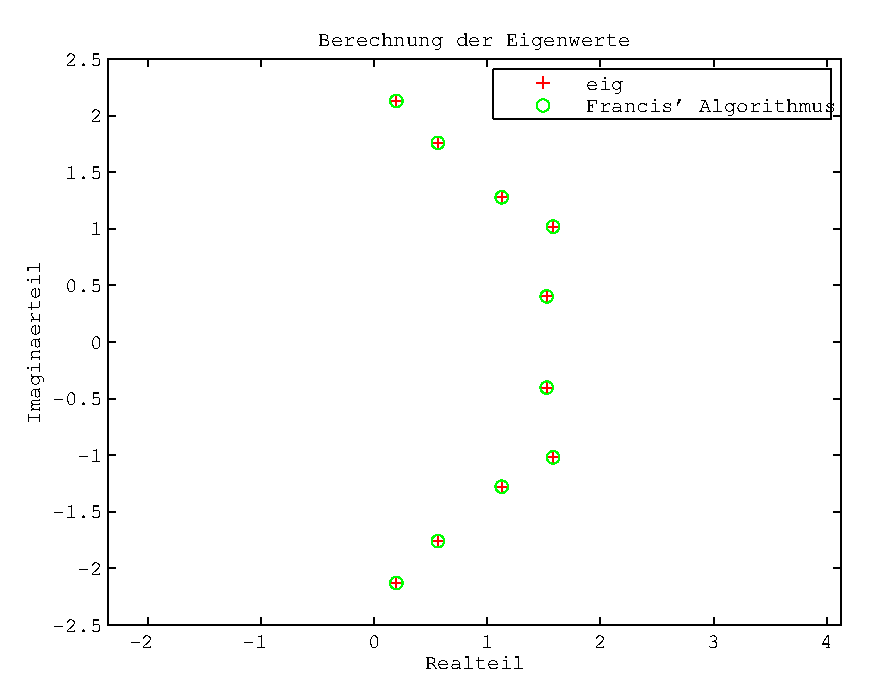
\includegraphics[width=\textwidth]{pics/Eigenwerte}
  \caption{\label{Abb:Eigenwerte} Eigenwerte einer Grcar-Matrix,
    berechnet mit der eingebauten Funktion \texttt{eig} und mit dem
    angegebenen Algorithmus nach Francis.}
\end{figure}

Wenn Ihnen die Programme als zu kompliziert und unverständlich
erscheinen: sämtliche fett gedruckten Begriffe sind vordefinierte
Befehle in \textsc{Matlab}, zu denen Sie sich die Hilfe mittels
\begin{quotation}
  \texttt{help} \textsf{<Begriff>}
\end{quotation}
anzeigen lassen können.

Natürlich können wir auch
\hyperref[alg:CGS]{Algorithmus~\ref*{alg:CGS}} in \textsc{Matlab}
implementieren, hier ist das Ergebnis:

\lstinputlisting[caption=Implementation des klassischen
Gram-Schmidt'schen\label{Prog:CGS}
Orthonormalisierungsverfahrens]{matlab/KlassischesGramSchmidtVerfahren.m}

Ein Beispiel zur Verwendung des Programms nebst Ausgabe finden Sie
hier:
\begin{verbatim}
>> A = [2 2;2 1;1 0]
A =
     2     2
     2     1
     1     0
>> [Q,R] = KlassischesGramSchmidtVerfahren(A)
Q =
     6.666666666666666e-01     6.666666666666667e-01
     6.666666666666666e-01    -3.333333333333333e-01
     3.333333333333333e-01    -6.666666666666666e-01
R =
     3     2
     0     1
>> Q*R
ans =
     2     2
     2     1
     1     0
>> Q'*Q
ans =
     1.000000000000000e+00     1.110223024625157e-16
     1.110223024625157e-16     1.000000000000000e+00
\end{verbatim}
Sie sehen, dass das Programm das Gewünschte leistet, wenn auch bei der
letzten Ausgabe zu sehen ist, dass \textsc{Matlab} numerisch rechnet,
also mit Fließkommazahlen, und daher Rundungsfehler macht. Die
sogenannte \emph{Maschinengenauigkeit} beschreibt den halben Abstand
von der Eins zu nächsten Fließkommazahl, in IEEE~754-Arithmetik ist
das $2^{-53}\approx1.110223024625157\cdot10^{-16}$. Bei Zahlen in der
Größenordnung von Eins (haben wir) ist also ein Fehler in der
Größenordnung von $10^{-16}$ zu erwarten (haben wir).

\section{Aufbau der Ausarbeitung}

Die von Ihnen zu erstellende Ausarbeitung sollte in einem ersten
Abschnitt
\begin{enumerate}
\item in das Thema adäquat einführen ($\leadsto$ Einführung),
\item die behandelten Themen motivieren ($\leadsto$ Motivation),
\item die verwendete Notation erläutern ($\leadsto$ Notation).
\end{enumerate}
Im folgenden Abschnitt/in den folgenden Abschnitten sollten die
wesentlichen Gedanken erläutert werden. In einem gesonderten Abschnitt
durch numerische Beispiele untermauert werden. Den Abschluss bildet
ein Fazit nebst eventuell einem Ausblick auf weitere Themen.

Somit sieht ein mögliches Inhaltsverzeichnis wie folgt aus:
\begin{enumerate}
\item Einführung
  \begin{enumerate}
  \item Motivation
  \item Notation
  \end{enumerate}
\item Die wesentliche Idee 1
\item Die wesentliche Idee 2
\item Numerische Beispiele
\item Fazit
\item Literaturverzeichnis
\end{enumerate}

In jedem einzelnen Satz sollten Sie klarstellen, ob die dort
aufgestellte Behauptung von Ihnen stammt, oder ob Sie bloß
zitieren. Wenn Sie zitieren, dann immer unter Angabe der Quelle. Das
können Sie in \LaTeX\ zum Beispiel in der Form
\begin{quotation}
  Watkins~\cite[Seite~18]{Watkins:2002} behauptet, dass viele
  physikalische Phänomene durch Differentialgleichungen modelliert
  werden können.
\end{quotation}
Wenn die Aussage zum Beispiel falsch ist, sind Sie als Autor auf der
sicheren Seite. Außerdem heimsen Sie so nicht die Lorbeeren für die
Arbeit eines Anderen ein, was niemand gerne sieht ($\leadsto$
Plagiat). Andererseits sollten Sie in der Einführung Ihren Anteil an
den erzielten Ergebnissen klarstellen (auch wenn in der Ausarbeitung
vermutlich eher wenig von Ihnen sein wird). Es gibt auch korrekte
Wege, Hilfsmittel wie Wikipedia und das große weite Internet zu
zitieren, siehe zum Beispiel
\begin{quotation}
  \url{https://de.wikipedia.org/wiki/Zitieren_von_Internetquellen}.
\end{quotation}
Allgemein ist das Zitieren von Internetquellen nicht beliebt, man
sollte versuchen sich auf gut verfügbare Quellen zu beschränken,
welche in klassischer Form daherkommen, wie Lehrbücher oder in
wissenschaftlichen Journalen publizierte Artikel.

\addcontentsline{toc}{section}{Literaturverzeichnis}%
\bibliographystyle{plain}
\bibliography{Proseminar}

\end{document}

%%% Local Variables: 
%%% mode: latex
%%% TeX-master: t
%%% End: 
